%===============================================================================
% LaTeX sjabloon voor de bachelorproef toegepaste informatica aan HOGENT
% Meer info op https://github.com/HoGentTIN/latex-hogent-report
%===============================================================================

\documentclass[dutch,dit,thesis]{hogentreport}

% TODO:
% - If necessary, replace the option `dit`' with your own department!
%   Valid entries are dbo, dbt, dgz, dit, dlo, dog, dsa, soa
% - If you write your thesis in English (remark: only possible after getting
%   explicit approval!), remove the option "dutch," or replace with "english".

\usepackage{lipsum} % For blind text, can be removed after adding actual content

%% Pictures to include in the text can be put in the graphics/ folder
\graphicspath{{graphics/}}

%% For source code highlighting, requires pygments to be installed
%% Compile with the -shell-escape flag!
\usepackage[section]{minted}
\usemintedstyle{solarized-light}
\definecolor{bg}{RGB}{253,246,227} %% Set the background color of the codeframe

%% Change this line to edit the line numbering style:
\renewcommand{\theFancyVerbLine}{\ttfamily\scriptsize\arabic{FancyVerbLine}}

%% Macro definition to load external java source files with \javacode{filename}:
\newmintedfile[javacode]{java}{
    bgcolor=bg,
    fontfamily=tt,
    linenos=true,
    numberblanklines=true,
    numbersep=5pt,
    gobble=0,
    framesep=2mm,
    funcnamehighlighting=true,
    tabsize=4,
    obeytabs=false,
    breaklines=true,
    mathescape=false
    samepage=false,
    showspaces=false,
    showtabs =false,
    texcl=false,
}

% Other packages not already included can be imported here

%%---------- Document metadata -------------------------------------------------
% TODO: Replace this with your own information
\author{Ernst Aarden}
\supervisor{Dhr. F. Van Houte}
\cosupervisor{Mevr. S. Beeckman}
\title[Optionele ondertitel]%
    {Titel van de bachelorproef}
\academicyear{\advance\year by -1 \the\year--\advance\year by 1 \the\year}
\examperiod{1}
\degreesought{\IfLanguageName{dutch}{Professionele bachelor in de toegepaste informatica}{Bachelor of applied computer science}}
\partialthesis{false} %% To display 'in partial fulfilment'
%\institution{Internshipcompany BVBA.}

%% Add global exceptions to the hyphenation here
\hyphenation{back-slash}

%% The bibliography (style and settings are  found in hogentthesis.cls)
\addbibresource{bachproef.bib}            %% Bibliography file
\addbibresource{../voorstel/voorstel.bib} %% Bibliography research proposal
\defbibheading{bibempty}{}

%% Prevent empty pages for right-handed chapter starts in twoside mode
\renewcommand{\cleardoublepage}{\clearpage}

\renewcommand{\arraystretch}{1.2}

%% Content starts here.
\begin{document}

%---------- Front matter -------------------------------------------------------

\frontmatter

\hypersetup{pageanchor=false} %% Disable page numbering references
%% Render a Dutch outer title page if the main language is English
\IfLanguageName{english}{%
    %% If necessary, information can be changed here
    \degreesought{Professionele Bachelor toegepaste informatica}%
    \begin{otherlanguage}{dutch}%
       \maketitle%
    \end{otherlanguage}%
}{}

%% Generates title page content
\maketitle
\hypersetup{pageanchor=true}

%%=============================================================================
%% Voorwoord
%%=============================================================================

\chapter*{\IfLanguageName{dutch}{Woord vooraf}{Preface}}%
\label{ch:voorwoord}

%% TODO:
%% Het voorwoord is het enige deel van de bachelorproef waar je vanuit je
%% eigen standpunt (``ik-vorm'') mag schrijven. Je kan hier bv. motiveren
%% waarom jij het onderwerp wil bespreken.
%% Vergeet ook niet te bedanken wie je geholpen/gesteund/... heeft

\lipsum[1-2]
%%=============================================================================
%% Samenvatting
%%=============================================================================

% TODO: De "abstract" of samenvatting is een kernachtige (~ 1 blz. voor een
% thesis) synthese van het document.
%
% Een goede abstract biedt een kernachtig antwoord op volgende vragen:
%
% 1. Waarover gaat de bachelorproef?
% 2. Waarom heb je er over geschreven?
% 3. Hoe heb je het onderzoek uitgevoerd?
% 4. Wat waren de resultaten? Wat blijkt uit je onderzoek?
% 5. Wat betekenen je resultaten? Wat is de relevantie voor het werkveld?
%
% Daarom bestaat een abstract uit volgende componenten:
%
% - inleiding + kaderen thema
% - probleemstelling
% - (centrale) onderzoeksvraag
% - onderzoeksdoelstelling
% - methodologie
% - resultaten (beperk tot de belangrijkste, relevant voor de onderzoeksvraag)
% - conclusies, aanbevelingen, beperkingen
%
% LET OP! Een samenvatting is GEEN voorwoord!

%%---------- Nederlandse samenvatting -----------------------------------------
%
% TODO: Als je je bachelorproef in het Engels schrijft, moet je eerst een
% Nederlandse samenvatting invoegen. Haal daarvoor onderstaande code uit
% commentaar.
% Wie zijn bachelorproef in het Nederlands schrijft, kan dit negeren, de inhoud
% wordt niet in het document ingevoegd.

\IfLanguageName{english}{%
\selectlanguage{dutch}
\chapter*{Samenvatting}
\lipsum[1-4]
\selectlanguage{english}
}{}

%%---------- Samenvatting -----------------------------------------------------
% De samenvatting in de hoofdtaal van het document

\chapter*{\IfLanguageName{dutch}{Samenvatting}{Abstract}}

In deze bachelorproef wordt er onderzocht welke anti-webscraping technieken er onder meer bestaan en hoe effectief deze zijn voor het stoppen van webscraping. \newline 
De initiële fase van het onderzoek bestaat uit een studie over de gebruikte methoden om data van websites te scrapen.
In de opvolgende fase zal er een vergelijkende studie uitgevoerd worden over de effectiviteit van bestaande anti-webscrapings technieken. Hierbij zal er nagegaan worden hoe deze methoden standhouden tegen de werking van de methodieken van de vorige fase.
Vervolgens wordt er onderzocht hoe deze technieken invloed hebben op de werking van de website en de gebruikerservaring.
\newline
Dit onderzoek is relevant omdat data een heel waardevolle rol speelt bij bedrijven. Juist omdat dit zo waardevol is, wordt er ook veel belang gehecht aan het beschermen ervan tegen concurrenten. Maar de meest effectieve oplossing is niet altijd de beste, het is ook belangrijk dat deze implementaties geen al te negatieve effecten hebben tegenover de klanten en gebruikers. Door de effectiviteit en impacten in kaart te brengen van verschillende beschermingstechnieken, kan er een accuratere beslissing gemaakt worden over welke techniek(-en) er geïmplementeerd moeten worden. Dit zorgt dan weer voor een uitsparing van tijd en budget voor bepaalde bedrijven die de  informatie op hun website wensen te beschermen.


%---------- Inhoud, lijst figuren, ... -----------------------------------------

\tableofcontents

% In a list of figures, the complete caption will be included. To prevent this,
% ALWAYS add a short description in the caption!
%
%  \caption[short description]{elaborate description}
%
% If you do, only the short description will be used in the list of figures

\listoffigures

% If you included tables and/or source code listings, uncomment the appropriate
% lines.
%\listoftables
%\listoflistings

% Als je een lijst van afkortingen of termen wil toevoegen, dan hoort die
% hier thuis. Gebruik bijvoorbeeld de ``glossaries'' package.
% https://www.overleaf.com/learn/latex/Glossaries

%---------- Kern ---------------------------------------------------------------

\mainmatter{}

% De eerste hoofdstukken van een bachelorproef zijn meestal een inleiding op
% het onderwerp, literatuurstudie en verantwoording methodologie.
% Aarzel niet om een meer beschrijvende titel aan deze hoofdstukken te geven of
% om bijvoorbeeld de inleiding en/of stand van zaken over meerdere hoofdstukken
% te verspreiden!

%%=============================================================================
%% Inleiding
%%=============================================================================

\chapter{\IfLanguageName{dutch}{Inleiding}{Introduction}}%
\label{ch:inleiding}

De inleiding moet de lezer net genoeg informatie verschaffen om het onderwerp te begrijpen en in te zien waarom de onderzoeksvraag de moeite waard is om te onderzoeken. In de inleiding ga je literatuurverwijzingen beperken, zodat de tekst vlot leesbaar blijft. Je kan de inleiding verder onderverdelen in secties als dit de tekst verduidelijkt. Zaken die aan bod kunnen komen in de inleiding~\autocite{Pollefliet2011}:

\begin{itemize}
  \item context, achtergrond
  \item afbakenen van het onderwerp
  \item verantwoording van het onderwerp, methodologie
  \item probleemstelling
  \item onderzoeksdoelstelling
  \item onderzoeksvraag
  \item \ldots
\end{itemize}

\section{\IfLanguageName{dutch}{Probleemstelling}{Problem Statement}}%
\label{sec:probleemstelling}

Uit je probleemstelling moet duidelijk zijn dat je onderzoek een meerwaarde heeft voor een concrete doelgroep. De doelgroep moet goed gedefinieerd en afgelijnd zijn. Doelgroepen als ``bedrijven,'' ``KMO's'', systeembeheerders, enz.~zijn nog te vaag. Als je een lijstje kan maken van de personen/organisaties die een meerwaarde zullen vinden in deze bachelorproef (dit is eigenlijk je steekproefkader), dan is dat een indicatie dat de doelgroep goed gedefinieerd is. Dit kan een enkel bedrijf zijn of zelfs één persoon (je co-promotor/opdrachtgever).

\section{\IfLanguageName{dutch}{Onderzoeksvraag}{Research question}}%
\label{sec:onderzoeksvraag}

Wees zo concreet mogelijk bij het formuleren van je onderzoeksvraag. Een onderzoeksvraag is trouwens iets waar nog niemand op dit moment een antwoord heeft (voor zover je kan nagaan). Het opzoeken van bestaande informatie (bv. ``welke tools bestaan er voor deze toepassing?'') is dus geen onderzoeksvraag. Je kan de onderzoeksvraag verder specifiëren in deelvragen. Bv.~als je onderzoek gaat over performantiemetingen, dan 

\section{\IfLanguageName{dutch}{Onderzoeksdoelstelling}{Research objective}}%
\label{sec:onderzoeksdoelstelling}

Wat is het beoogde resultaat van je bachelorproef? Wat zijn de criteria voor succes? Beschrijf die zo concreet mogelijk. Gaat het bv.\ om een proof-of-concept, een prototype, een verslag met aanbevelingen, een vergelijkende studie, enz.

\section{\IfLanguageName{dutch}{Opzet van deze bachelorproef}{Structure of this bachelor thesis}}%
\label{sec:opzet-bachelorproef}

% Het is gebruikelijk aan het einde van de inleiding een overzicht te
% geven van de opbouw van de rest van de tekst. Deze sectie bevat al een aanzet
% die je kan aanvullen/aanpassen in functie van je eigen tekst.

De rest van deze bachelorproef is als volgt opgebouwd:

In Hoofdstuk~\ref{ch:stand-van-zaken} wordt een overzicht gegeven van de stand van zaken binnen het onderzoeksdomein, op basis van een literatuurstudie.

In Hoofdstuk~\ref{ch:methodologie} wordt de methodologie toegelicht en worden de gebruikte onderzoekstechnieken besproken om een antwoord te kunnen formuleren op de onderzoeksvragen.

% TODO: Vul hier aan voor je eigen hoofstukken, één of twee zinnen per hoofdstuk

In Hoofdstuk~\ref{ch:conclusie}, tenslotte, wordt de conclusie gegeven en een antwoord geformuleerd op de onderzoeksvragen. Daarbij wordt ook een aanzet gegeven voor toekomstig onderzoek binnen dit domein.
\chapter{\IfLanguageName{dutch}{Stand van zaken}{State of the art}}%
\label{ch:stand-van-zaken}

% Tip: Begin elk hoofdstuk met een paragraaf inleiding die beschrijft hoe
% dit hoofdstuk past binnen het geheel van de bachelorproef. Geef in het
% bijzonder aan wat de link is met het vorige en volgende hoofdstuk.

\paragraph{Inleiding}

\textbf{TODO:}
\\ 
achterliggende structuur webapplicatie uitleggen, Jhipster toevoegen en uitleg hiervan, SEO en ranking uitleggen, \textbf{note:} Leg ik best hier al gedetailleerder uit hoe de webscraping en antiwebscrapingstechnieken a.d.h.v gedetaillerdere voorbeelden of laat ik het zo met een gewone tekstuitleg en de voorbeelden pas aanhalen in mijn methodologie? Want ik wou dit dan ook doen aan de hand van de demoapplicatie maar hier is daar dan nog niets opgezet. Maar langs de andere kant is het nu vaak nog al onduidelijk/vaag uitgelegd is hoe technieken werken maar ga ik anders ook niet veel dubbel staan hebben in mijn methodologie? Weet niet zo goed wat te doen aangezien het zo wat dubbel is.

In dit hoofdstuk zal er meer informatie gegeven worden over wat web scraping is, hoe het werkt en wat de huidige maatregelen tegen web scraping zijn. 
\textbf{Note:} Zet ik hierin de litertuurstudie best ook extra informatie over hoe ik verwacht hoe de anti web scrapingstechnieken invloed zullen hebben op de performance? een voorbeeld hiervan is dat ik verwacht dat bij dynamische generatie, de pagina's veel trager gaan laden doordat er niet aan caching gedaan kan worden omdat de pagina altijd veranderd van structuur ==> geef ik hierbij dan meer info in de literatuurstudie over hoe de caching werkt?  
% Pas na deze inleidende paragraaf komt de eerste sectiehoofding.

\section{Terminologie}

\textbf{Note:}
\\ Hoort terminologie hier thuis? of moet dit eigenlijk in een andere sectie staan?

\subsection{HTTP protocol} \label{HTTP protocol}
Het Hypertext Transfer Protocol is een applicatie-level protocol dat gebruikt wordt bij distributed collaboratieve hypermedia informatiesystemen. Dit protocol dient om dataoverdracht te voorzien over het internet aan de hand van HTTP messages(zie \ref{HTTP message}) (\cite{rfc2616}). 
\subsection{HTTP message}\label{HTTP message}
Dit is de basiseenheid van HTTP communicatie en is opgebouwd uit de startlijn, header(-s)(zie \ref{Message header}), een lege lijn om het einde van de header(-s) aan te duiden en een eventuele message-body (\cite{rfc2616}).
\subsection{Message header} \label{Message header}
Een header wordt aanzien als een key-value pair om informatie mee te geven (\cite{rfc2616}).
\subsection{HTTP request} \label{HTTP request}
Een HTTP request message van een cliënt naar een server (\cite{rfc2616}).
\subsection{HTTP response} \label{HTTP response}
Een HTTP response message van een server naar een client nadat een request message geïnterpreteerd is (\cite{rfc2616}).
\subsection{Reguliere expressie} \label{Reguliere expressie}
Een reguliere expressies is een sequentie van karakters dat gebruikt wordt door de compiler als input. Vervolgens gaat de compiler een signaal geven elke keer als een string in de tekst overeenkomt met de reguliere expressie.  (\cite{10.1145/363347.363387})
\subsection{CSS Selectors} \label{css selectors}
CSS selectors zijn patronen die gebruikt worden om HTML elementen te selecteren gebaseerd op CSS properties zoals id, class, type, etc. (\cite{Persson2019}).


\section{Web scraping} \label{Web scraping}
In theorie is web scraping, ook bekend als web extraction of harvesten, de activiteit van het verzamelen van gegevens op een andere manier dan via API calls of menselijke interactie. Dit gebeurt meestal door het schrijven van een programma dat een website raadpleegt, gegevens opvraagt waaruit webpagina's bestaan, en die gegevens vervolgens verwerkt om er de benodigde informatie uit te halen en op te slagen in een bestand of database om deze vervolgens later op te vragen of te analyseren (\cite{Mitchell2018,Zhao2017}).
\\
\\
Web scraping is opgebouwd uit 3 verschillende fases, namelijk ophaling van data, extractie van data en transformatie van data. 
\begin{enumerate}
    \item \textbf{Ophaling van data}
\\
In deze fase moet de gewenste website bereikt worden aan de hand van het HTTP protocol (zie \ref{HTTP protocol}). De effectieve ophaling van data gebeurd  door een library die een HTTP GET request zal sturen naar een bepaalde URL en vervolgens de bijhorende webpagina terugkrijgt als een HTML document via de response ( \cite{Persson2019}).
    \item \textbf{Extractie van data}
\\
Bij deze fase wordt de data die gewenst is geëxtraheerd uit het HTML document verkregen in vorige fase. Dit gebeurd meestal aan de hand van REGEX, HTML parsing libraries of XPath queries om de gewenste data te vinden (\cite{Persson2019}).
    \item \textbf{Transformatie van data}
\\
Hierbij wordt de data die geëxtraheerd is getransformeerd in een gestructureerde versie (\cite{Persson2019}).
\end{enumerate}

\subsection{Web scraping methodes}
Niet alle web scraping libraries en frameworks benaderen de extractie van data op dezelfde manier. Zo bestaan er verschillende methoden om dit aan te pakken, zoals:
\begin{itemize}
    \item \textbf{Text Pattern Matching}
\\
Text pattern matching maakt gebruikt van reguliere expressies (zie \ref{Reguliere expressie}) om aan de hand van een patroon de gewenste tekst terug te vinden in het overkoepelend document. In deze paper gaat er niet verder worden ingegaan op text pattern matching aangezien de mogelijkheden van deze methode best beperkt zijn. (\textbf{Note} kan eventueel nog veranderen aangezien regex misschien als ondersteunende methode gebruikt gaat worden bij HTML parsing en dom parsing).
    \item \textbf{HTML Parsing a.d.h.v CSS selectors}
\\
Deze methode maakt gebruikt van de CSS selectors(zie \ref{css selectors}) om data te extraheren uit HTML documenten. Hierbij kan er gezocht worden op e.g. id's en klassen om de juiste data terug te vinden. (\cite{Persson2019})
\\
Om een voorbeeld te geven van hoe deze methode toegepast wordt, gaat er gebruik gemaakt worden van de HTML pagina gebaseerd op de code in figuur \ref{fig:figuur 1.1.png}. Stel nu dat de 3de heading de gewenste data omvat, kan er in dit geval HTML Parsing toegepast worden a.d.h.v de 'id' css selector. In dit specifiek geval zal vervolgens de tekst in '3de Heading' teruggeven worden.
\\

    \item \textbf{DOM Parsing}
In tegenstelling tot HTML parsing gaat DOM Parsing zich focussen op XPath (XML Path Language)  i.p.v css selectors. Xpath is een query taal dat gebruikt wordt om te navigeren in XML documenten en daarin eventueel selecties te maken. Xpath kan ook gebruikt worden om te navigeren in HTML documenten aangezien deze ook gebruik maken van de XML boomstructuur. (\cite{Persson2019,Mitchell2018})
\\
Om de werking van deze methode te tonen zal er weer gebruik gemaakt worden van de HTML pagina gebaseerd op de code in figuur \ref{fig:figuur 1.1.png}. Om het Xpath terug te vinden van de  3de heading voor DOM parsing moet er  gekeken worden naar de boomstructuur. In dit geval bevind deze header zich onder de <body> tag die zich vervolgens onder de <html> tag bevind. Afgeleid van deze informatie zal het Xpath van de 3de heading neerkomen op 
"/html/body/h1[3]". Dit resultaat kan vervolgens gebruikt worden om de tekst van de 3de Heading terug te geven.
    \item \textbf{Pagina analyse a.d.h.v computer visie en A.I}
Deze methode van web scraping kan vooral gebruikt in situaties waar de DOM obscuur is en vaak ge-update wordt maar de visuele structuur van de webpagina hetzelfde blijft. De gedachtegang voor deze methode is om een machine learning model te gaan trainen op gelabelde screenshots van een gelijkaardige website waarvan er wel makkelijk gescraped kan worden (e.g. webshop structuren zijn in het algemeen heel overeenkomend) of zelf een mock-up met mock-data op te zetten. Vervolgens wordt er a.d.h.v selenium aan screen capture gedaan van de gewenste te scrapen webpagina's en in real time geëvalueerd door het model en de gewenste data wordt uit deze foto's gehaald (bv. productnamen, product id's en prijzen bij een webshop). 
\\
\textbf{Note }van deze uitwerking heb ik geen effectieve goede bronnen van terug gevonden maar ik weet dat zulke services wel bestaan (https://www.diffbot.com/). Dit is eerder een gedachte van nog eventueel zelf uit te werken als ik hier de tijd voor heb maar leek me wel interessant om hier voorlopig bij te zetten en eventueel erna te verwijderen of effectief uit te werken. Maar aangezien ik hier geen bron van heb en dit mijn eigen gedachtengang is moet dit waarschijnlijk eerder bij de uitwerking?)
\end{itemize}

\begin{figure}[b]
    \centering
    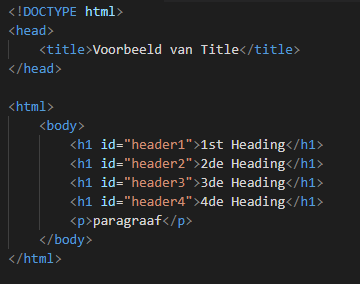
\includegraphics{bachproef/graphics/figuur 1.1.png}
    \caption{Voorbeeld van een simpele webpagina}
    \label{fig:figuur 1.1.png}
\end{figure}

\section{Anti web scraping methodes}
Zoals aangehaald in de paper \cite{10.1007/978-3-030-90016-8_4} is er een als maar stijgende vraag voor nieuwe en bruikbare data. Deze data wordt vaak niet manueel opgehaald maar hiervoor worden de vooraf aangehaalde methoden in sectie \ref{Web scraping} gebruikt, of specifieker de libraries en frameworks dat onderliggend gebruik maken van deze methoden. Om deze reden is het dan ook belangrijk om deze tegen te kunnen gaan. Zo bestaan er verschillende technieken om dit te bereiken, een paar voorbeelden aangehaald door \autocite{10.1007/978-3-030-90016-8_4} zijn:
\begin{itemize}
    \item \textbf{Rate limiting} 
    \\
Rate limiting werkt aan de hand van de snelheid van verzoeken op een website te beperken. Hierdoor kunnen web scraping programma's maar een bepaald aantal requests sturen naar de web server voordat ze buitengesloten worden.
    \item \textbf{Herkennen van automatisch netwerkverkeer} 
    \\
Deze techniek gaat zich eerder focussen naar het verwerken van informatie over het netwerkverkeer.
Dit is nu eenmaal mogelijk omdat web scrapers zich niet hetzelfde gedragen zoals humane gebruikers. 

Een paar indicatoren van web scrapers die gebruikt kunnen worden om hun buiten te sluiten zijn bijvoorbeeld:
\item Een hoog aantal paginabezoeken van hetzelfde ip-adres op een korte tijd
\item Een korte duratie van paginabezoeken aangezien web scrapers praktisch direct alle informatie verkrijgen van een webpagina en deze dan ook direct weer sluiten
\item  Netwerkverkeer uit landen dat onlogisch is. Lokale bedrijven gaan geen hoog aantal paginabezoeken krijgen uit landen aan de andere kant van de wereld. Dit duidt dan ook regelmatig op web scrapers. 
\item Een hoog aantal clicks op links die onlogisch lijken. Bv. leeg ingevulde contactformulieren, gebruikers die alle artikels in een webshop in hun winkelmandje plaatsen, etc.
\item Vreemde user-agents uitfilteren \textbf{Note: hier nog dieper op ingaan hoe user-agents werken, hoe ze er normaal moeten uitzien en hoe we vreemde user-agents kunnen vinden}
    
\item \textbf{Honey potting}
\\
Deze tactiek werkt door het strategisch plaatsen van  links of knoppen waardoor alleen bots ze kunnen vinden en gebruiken.
\textbf{}
\\
\\
Naast de voorbeelden uit de paper \cite{10.1007/978-3-030-90016-8_4} bestaan er nog verscheidene andere technieken die zullen uitgewerkt worden:
\item Dynamisch genereren van random id's en klassen. Door dit te randomiseren kan er geen gebruik gemaakt worden van bepaalde CSS selectors.
\item Dynamisch div's encapsuleren zodat de boomstructuur telkens veranderd. Op deze manier zal er ook geen mogelijkheid zijn om gebruik te maken van DOM parsing.
\item Tekst op de webpagina's tonen als foto.
\item Javascript gebruiken om de paginacontent te laden. Dit zorgt ervoor dat HTML parsers niet meer werken aangezien deze geen javascript runnen.
\end{itemize}



%Dit hoofdstuk bevat je literatuurstudie. De inhoud gaat verder op de inleiding, maar zal het onderwerp van de bachelorproef *diepgaand* uitspitten. De bedoeling is dat de lezer na lezing van dit hoofdstuk helemaal op de hoogte is van de huidige stand van zaken (state-of-the-art) in het onderzoeksdomein. Iemand die niet vertrouwd is met het onderwerp, weet nu voldoende om de rest van het verhaal te kunnen volgen, zonder dat die er nog andere informatie moet over opzoeken \autocite{Pollefliet2011}.

%Je verwijst bij elke bewering die je doet, vakterm die je introduceert, enz.\ naar je bronnen. In \LaTeX{} kan dat met het commando \texttt{$\backslash${textcite\{\}}} of \texttt{$\backslash${autocite\{\}}}. Als argument van het commando geef je de ``sleutel'' van een ``record'' in een bibliografische databank in het Bib\LaTeX{}-formaat (een tekstbestand). Als je expliciet naar de auteur verwijst in de zin, gebruik je \texttt{$\backslash${}textcite\{\}}.
%Soms wil je de auteur niet expliciet vernoemen, dan gebruik je \texttt{$\backslash${}autocite\{\}}. In de volgende paragraaf een voorbeeld van elk.

%\textcite{Knuth1998} schreef een van de standaardwerken over sorteer- en zoekalgoritmen. Experten zijn het erover eens dat cloud computing een interessante opportuniteit vormen, zowel voor gebruikers als voor dienstverleners op vlak van informatietechnologie~\autocite{Creeger2009}.

%\lipsum[7-20]

%%=============================================================================
%% Methodologie
%%=============================================================================

\chapter{\IfLanguageName{dutch}{Methodologie}{Methodology}}%
\label{ch:methodologie}

%% TODO: Hoe ben je te werk gegaan? Verdeel je onderzoek in grote fasen, en
%% licht in elke fase toe welke stappen je gevolgd hebt. Verantwoord waarom je
%% op deze manier te werk gegaan bent. Je moet kunnen aantonen dat je de best
%% mogelijke manier toegepast hebt om een antwoord te vinden op de
%% onderzoeksvraag.

\lipsum[21-25]



% Voeg hier je eigen hoofdstukken toe die de ``corpus'' van je bachelorproef
% vormen. De structuur en titels hangen af van je eigen onderzoek. Je kan bv.
% elke fase in je onderzoek in een apart hoofdstuk bespreken.

%\input{...}
%\input{...}
%...

%%=============================================================================
%% Conclusie
%%=============================================================================

\chapter{Conclusie}%
\label{ch:conclusie}

% TODO: Trek een duidelijke conclusie, in de vorm van een antwoord op de
% onderzoeksvra(a)g(en). Wat was jouw bijdrage aan het onderzoeksdomein en
% hoe biedt dit meerwaarde aan het vakgebied/doelgroep? 
% Reflecteer kritisch over het resultaat. In Engelse teksten wordt deze sectie
% ``Discussion'' genoemd. Had je deze uitkomst verwacht? Zijn er zaken die nog
% niet duidelijk zijn?
% Heeft het onderzoek geleid tot nieuwe vragen die uitnodigen tot verder 
%onderzoek?

\lipsum[76-80]



%---------- Bijlagen -----------------------------------------------------------

\appendix

\chapter{Onderzoeksvoorstel}

Het onderwerp van deze bachelorproef is gebaseerd op een onderzoeksvoorstel dat vooraf werd beoordeeld door de promotor. Dat voorstel is opgenomen in deze bijlage.

%% TODO: 
%\section*{Samenvatting}

% Kopieer en plak hier de samenvatting (abstract) van je onderzoeksvoorstel.

% Verwijzing naar het bestand met de inhoud van het onderzoeksvoorstel
%---------- Inleiding ---------------------------------------------------------

\section{Introductie}%
\label{sec:introductie}

Web scraping maakt het mogelijk om snel een grote hoeveelheid gegevens van websites te verzamelen en te verwerken. Daarnaast is het ook zeer tijdsefficiënt, waardoor gegevens van verschillende bronnen automatisch kunnen worden verzameld, terwijl dit voorheen een moeizame handmatige inspanning vergde ~(\cite{NYLEN2017277}). Dit zorgt dan ook voor een probleem bij verscheidene bedrijven, aangezien niet elk bedrijf wilt dat hun data automatisch verkrijgbaar is, zo willen online winkels bijvoorbeeld niet dat hun concurrenten alle prijzen kunnen verzamelen om hun eigen prijzen daarop te baseren. Anti-webscrapingstechnieken kunnen hierbij een oplossing bieden waardoor data manueel verzameld zal moeten worden in plaats van automatisch. De doelstelling van deze thesis is dan ook een inzicht te geven in welke technieken het beste passen in een bepaalde situatie (gebruikerservaring/prestaties over effectiviteit of omgekeerd). Daarnaast is in deze bachelorproef er ook voor gekozen om de focus te leggen op het beschermen van webshops.
\newline
In deze thesis zal de volgende onderzoeksvraag uitgewerkt worden met bijhorende deelvragen:
\begin{itemize}
\item In welke mate is het mogelijk om een website te beschermen tegen de gekende technieken van web scraping en hoe beïnvloeden deze de website?
    \begin{itemize}
    \item Hoe beïnvloeden anti-webscrapingstech- nieken de gebruikerservaring?
    \item Hoe beïnvloeden anti-webscrapingstech- nieken de performance van de website?
    \item Hoe beïnvloeden anti-webscrapingstech- nieken de Search Engine optimization van de website?
    \item Wat is op dit moment de meest effectieve oplossing los van de gevolgen?
    \end{itemize}
\end{itemize}
%---------- Stand van zaken ---------------------------------------------------

\section{State-of-the-art}%
\label{sec:state-of-the-art}
In deze sectie zal er meer informatie gegeven worden over wat web scraping is, hoe het werkt, welke methodes er bestaan en wat de huidige maatregelen tegen web scraping zijn.
\subsection{Wat is web scraping?}
Uit de studies van \cite{Mitchell2018,Zhao2017} kan er geconcludeerd worden dat in theorie web scraping, ook bekend als web extraction of
harvesten, de activiteit is van het verzamelen van gegevens op een andere manier dan via API calls of menselijke interactie. Dit gebeurt meestal door het schrijven van een geautomatiseerd programma dat een website raadpleegt, gegevens opvraagt waaruit webpagina's bestaan, en die gegevens vervolgens verwerkt om er de benodigde informatie uit te halen en op te slaan in een bestand of database om deze vervolgens later op te vragen of te analyseren  
\newline
Volgens \cite{Persson2019} is web scraping opgebouwd uit 3 verschillende fases, namelijk ophaling van data, extractie van data en transformatie van data.

\begin{enumerate}
    \item \textbf{Ophaling van data}
\\
In deze fase moet de gewenste website bereikt worden aan de hand van het HTTP protocol. De effectieve ophaling van data gebeurd  door een library die een HTTP GET request zal sturen naar een bepaalde URL en vervolgens de bijhorende webpagina terugkrijgt als een HTML document via de response.
    \item \textbf{Extractie van data}
\\
Bij deze fase wordt de data die gewenst is geëxtraheerd uit het HTML document verkregen in vorige fase. Dit gebeurd meestal aan de hand van REGEX, HTML parsing libraries of XPath queries om de gewenste data te vinden.
    \item \textbf{Transformatie van data}
\\
Hierbij wordt de data die geëxtraheerd is getransformeerd in een gestructureerde versie
\end{enumerate}

\subsection{Welke web scraping methodes bestaan er?}
Niet alle web scraping libraries en frameworks werken op dezelfde manier. Zo bestaan er verschillende methoden om dit aan te pakken, zoals:
\begin{itemize}
    \item \textbf{Text-pattern matching}
    \\
    Text pattern matching maakt gebruikt van reguliere expressies om aan de hand van een patroon de gewenste tekst terug te vinden in het overkoepelend document.
    \item \textbf{HTML parsing}
    \\
    Deze methode maakt gebruikt van de CSS selectors om data te extraheren uit HTML documenten. Hierbij kan er gezocht worden op e.g. id's en klassen om de juiste data terug te vinden. (\cite{Persson2019})
    \item \textbf{DOM parsing}
    \\ In tegenstelling tot HTML parsing gaat DOM Parsing zich focussen op XPath (XML Path Language)  i.p.v css selectors. Xpath is een query taal dat gebruikt wordt om te navigeren in XML documenten en daarin eventueel selecties te maken. Xpath kan ook gebruikt worden om te navigeren in HTML documenten aangezien deze ook gebruik maken van de XML boomstructuur. (\cite{Persson2019,Mitchell2018})
    \item \textbf{Pagina analyse a.d.h.v computer visie}
    \\
    Deze methode van web scraping kan vooral gebruikt in situaties waar de DOM obscuur is en vaak ge-update wordt maar de visuele structuur van de webpagina hetzelfde blijft. De gedachtegang voor deze methode is om een machine learning model te gaan trainen op gelabelde screenshots van een gelijkaardige website en deze vervolgens te gaan gebruiken op de "target" website om gewenste data op te halen.
\end{itemize}

\subsection{Waarom zou men dit willen tegengaan?}
\textbf{Note: deze sectie moet ik nog herschrijven naar een doorlopende tekst}
Een grote reden hiervoor is de gevolgen dat de webscrapers kunnen hebben op de website en het bedrijf: 
\begin{itemize}
    \item Geldverlies door mijden van advertenties \newline \autocite{Krotov2020}
    \item Het mogelijk maken voor concurrenten om prijzen en aanbiedingen te onderbieden, leidend tot minder verkoopcijfers
    \item Verspilling van tijd, geld en middelen door het creëren van originele inhoud die uiteindelijk elders wordt gedupliceerd
    \item Impact op de website prestaties eventueel leidende tot een denial of service(een bron (site, toepassing, server) die niet beschikbaar is voor het doel waarvoor hij is ontworpen)
    \item Misleidende dataverzameling door bezichtigingen van webscrapers (e.g websites dat datacollectie uitvoeren op hun gebruikers om te bepalen wat de meest/minst populaire artikels of producten zijn. Vervolgens  deze informatie gaan gebruiken om aanpassingen te maken naargelang hun behoeftes (bv. minst bezochte productpagina's gaan aanpassen om meer bezichtigingen te verkrijgen). Hierdoor kunnen de pagina's die regelmatig bezocht worden door een scraper onterecht beter scoren)
\end{itemize}

\subsection{Welke anti-webscrapingstechnie- ken bestaan er?}
Er bestaan verscheidene technieken om web scraping tegen te gaan, een paar voorbeelden aangehaald door \autocite{10.1007/978-3-030-90016-8_4} zijn:
\begin{itemize}
    \item \textbf{Rate limiting}
    \\
    De snelheid van verzoeken op een website beperken
    \item \textbf{Herkennen van automatisch netwerkverkeer}
    \\
    Deze techniek gaat zich eerder focussen naar het verwerken van informatie over het netwerkverkeer.
    \item \textbf{Toegang weigeren aan bekende malicieuze identificatoren}
    \\
    \item \textbf{Honey potting}
    \\
    Strategisch geplante links of knoppen waardoor alleen bots ze kunnen vinden en gebruiken
\end{itemize}

\subsection{Het probleem met deze informatie?}
In tegenstelling tot web scraping zelf zijn er zeer weinig academische bronnen te vinden over het beschermen van web applicaties tegen web scraping. Daarnaast zijn er nog verschillende technieken die niet aangehaald zijn in deze bronnen zoals:
\\
\begin{itemize}
\item Dynamisch genereren van random id's en klassen. Door dit te randomiseren kan er geen gebruik gemaakt worden van bepaalde CSS selectors.
\item Dynamisch div's encapsuleren zodat de boomstructuur telkens veranderd. Op deze manier zal er ook geen mogelijkheid zijn om gebruik te maken van DOM parsing.
\item Tekst op de webpagina's tonen als een foto.
\item Javascript gebruiken om de paginacontent te laden. Dit zorgt ervoor dat HTML parsers niet meer werken aangezien deze geen javascript runnen.
\end{itemize}

Het doel van dit onderzoek is dan ook om deze methodes uit te werken, te testen en de bevindingen te noteren. Daarnaast halen de bronnen ook niet aan hoe deze technieken een impact hebben op de gebruikers en de performance van de website.

% Voor literatuurverwijzingen zijn er twee belangrijke commando's:
% \autocite{KEY} => (Auteur, jaartal) Gebruik dit als de naam van de auteur
%   geen onderdeel is van de zin.
% \textcite{KEY} => Auteur (jaartal)  Gebruik dit als de auteursnaam wel een
%   functie heeft in de zin (bv. ``Uit onderzoek door Doll & Hill (1954) bleek
%   ...'')


%---------- Methodologie ------------------------------------------------------
\section{Methodologie}%
\label{sec:methodologie}
De eerste fase van het onderzoek gaat zich focussen op het opstellen van de demo-applicatie die verder in het onderzoek gebruikt wordt.
\newline
\break
Bij de opvolgende fase gaat er een literatuurstudie over de verscheidene webscrapingstechnieken en de daarop gebaseerde frameworks en libraries plaatsvinden.Daarnaast zal ook de werking van al deze technieken getoond worden op de demo-applicatie.
\newline
\break
Bij de derde fase zal er een empirisch onderstoek uitgevoerd
worden over de effectiviteit van bestaande anti-webscrapingstechnieken. Hierbij zal er nagegaan worden hoe
deze methoden standhouden tegen de werking van de meerdere concepten uit de vorige fase. De bedoeling is dan ook om al deze concepten uit te werken aan de hand van een proefopstelling.
\newline
\break
In de laatste fase gaat er onderzocht worden hoe de technieken uit de derde fase de prestaties van de website, de gebruikerservaring en de SEO beïnvloeden.Hieruit zullen vervolgens conclusies getrokken worden om de vooraf opgestelde onderzoeksvragen te beantwoorden.

\subsection{Technologieën}
Webscrapers kunnen gemaakt worden met verscheidene tools en programmeertalen. In deze paper zal er gebruik gemaakt worden van Python om deze op te stellen. Voor de testomgeving zal er gebruik gemaakt worden van HTML, CSS en JavaScript om een website op te maken. 

%---------- Verwachte resultaten ----------------------------------------------
\section{Verwacht resultaat, conclusie}%
\label{sec:verwachte_resultaten}
Er bestaat een mogelijkheid om (automatische) web scraping volledig tegen te gaan al zal er waarschijnlijk een combinatie van verscheidene technieken voor moeten gebruikt worden. 
Daarnaast zullen de meeste beschermingstechnieken op een of andere manier altijd wel een negatieve invloed hebben op de gebruikservaring. Bepaalde technieken zullen ook zorgen voor een slechtere leesbaarheid van de code en ook laadtijden, opslag, werking op mobiele apparaten en SEO ranking beïnvloeden.
\newline 

%%---------- Andere bijlagen --------------------------------------------------
% TODO: Voeg hier eventuele andere bijlagen toe. Bv. als je deze BP voor de
% tweede keer indient, een overzicht van de verbeteringen t.o.v. het origineel.
%\input{...}

%%---------- Backmatter, referentielijst ---------------------------------------

\backmatter{}

\setlength\bibitemsep{2pt} %% Add Some space between the bibliograpy entries
\printbibliography[heading=bibintoc]

\end{document}
